\let\negmedspace\undefined
\let\negthickspace\undefined
\documentclass[journal]{IEEEtran}
\usepackage[a5paper, margin=10mm, onecolumn]{geometry}
%\usepackage{lmodern} % Ensure lmodern is loaded for pdflatex
\usepackage{tfrupee} % Include tfrupee package

\setlength{\headheight}{1cm} % Set the height of the header box
\setlength{\headsep}{0mm}     % Set the distance between the header box and the top of the text

\usepackage{gvv-book}
\usepackage{gvv}
\usepackage{cite}
\usepackage{amsmath,amssymb,amsfonts,amsthm}
\usepackage{algorithmic}
\usepackage{graphicx}
\usepackage{textcomp}
\usepackage{xcolor}
\usepackage{txfonts}
\usepackage{listings}
\usepackage{enumitem}
\usepackage{mathtools}
\usepackage{gensymb}
\usepackage{comment}
\usepackage[breaklinks=true]{hyperref}
\usepackage{tkz-euclide} 
\usepackage{listings}
% \usepackage{gvv}                                        
\def\inputGnumericTable{}                                 
\usepackage[latin1]{inputenc}                                
\usepackage{color}                                            
\usepackage{array}                                            
\usepackage{longtable}                                       
\usepackage{calc}                                             
\usepackage{multirow}                                         
\usepackage{hhline}                                           
\usepackage{ifthen}                                           
\usepackage{lscape}
\begin{document}
\bibliographystyle{IEEEtran}
\renewcommand{\thefigure}{\theenumi}
\renewcommand{\thetable}{\theenumi}
\setlength{\intextsep}{10pt} % Space between text and floats
\numberwithin{equation}{enumi}
\numberwithin{figure}{enumi}
\renewcommand{\thetable}{\theenumi}
\title{1-1.9-22}

\author{AI24BTECH11016-Jakkula Adishesh Balaji}
\maketitle
\bigskip
\section*{\textbf{Vector Arithmetic(CBSE)}}
         \parindent 0px
         Question\brak{1.9.22}Find the value of y for which the distance between the points \textbf{P} $\brak{2,-3}$ and \textbf{Q} $\brak{10,y}$ is $10$ units. \\
	\solution
	\begin{table}[h!]
         	\centering
         	\begin{tabular}[12pt]{ |c| c|}
    \hline
    Parameter & Description\\ 
    \hline
    $P$ & $\myvec{2\\-3}$ \\
    \hline 
    $Q$ & $\myvec{10\\y}$ \\
    \hline
    $D$ & $Q-P$\\
    \hline 
    Distance & $10$ \\
    \hline
    \end{tabular}

         	\caption{Variables Used}
         	\label{tab1.9.22}
         \end{table}
	\begin{align}
	\norm{D}^2 &= 100 \\
	\norm{D}^{2} &= D{D}^{T} \\
	\norm{D}^{2} &= \myvec{8 & y+3}\myvec{8 \\ y+3} \\
       	100 &= 73 + y^{2} + 6y \\
 	\therefore y &= 3,-9 \\
	\end{align}
	\begin{figure}[h]
		\centering
		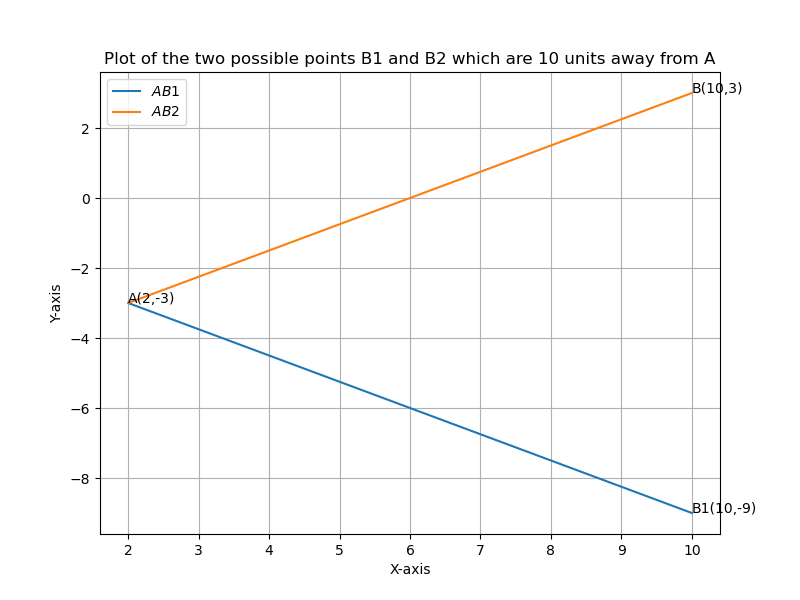
\includegraphics[scale=0.6]{figs/plot.png}
		\label{Fig}
	\end{figure}
\end{document}
